\documentclass[aspectratio=169]{beamer}

\usetheme{Boadilla}
\usefonttheme{professionalfonts}
\setbeamertemplate{navigation symbols}{}
\setbeamertemplate{itemize items}[circle]
\setbeamertemplate{enumerate items}[default]
\setbeamertemplate{headline}{}

\usepackage[utf8]{inputenc}
\usepackage[T1]{fontenc}
\usepackage{lmodern}
\usepackage{amsmath}
\usepackage{booktabs}
\usepackage{tabularx}
\usepackage{array}
\usepackage{hyperref}
\usepackage[strings]{underscore}
\usepackage{listings}
\usepackage{tikz}
\usetikzlibrary{arrows.meta,positioning,fit,calc,shapes.geometric}
\usepackage{xcolor}

\definecolor{courseblue}{HTML}{12355B}
\definecolor{coursegold}{HTML}{C98A2E}
\definecolor{courseice}{HTML}{EEF3F8}
\definecolor{coursegreen}{HTML}{2F6B4F}
\definecolor{coursegray}{HTML}{4B5563}
\definecolor{codebg}{HTML}{F7F9FC}
\definecolor{codecomment}{HTML}{5E6C84}
\definecolor{codestring}{HTML}{0B6E4F}

\setbeamercolor{palette primary}{bg=courseblue,fg=white}
\setbeamercolor{palette secondary}{bg=coursegold,fg=white}
\setbeamercolor{palette tertiary}{bg=courseblue,fg=white}
\setbeamercolor{palette quaternary}{bg=coursegold,fg=white}
\setbeamercolor{structure}{fg=courseblue}
\setbeamercolor{frametitle}{bg=courseice,fg=courseblue}
\setbeamercolor{title}{fg=courseblue}
\setbeamercolor{block title}{bg=courseblue,fg=white}
\setbeamercolor{block body}{bg=courseice,fg=black}
\setbeamercolor{normal text}{fg=black,bg=white}
\setbeamercolor{alerted text}{fg=coursegold}

\setbeamerfont{footline}{size=\scriptsize}

\setbeamertemplate{footline}{
  \leavevmode
  \hbox{
    \begin{beamercolorbox}[wd=.33\paperwidth,ht=2.8ex,dp=1.2ex,leftskip=0.8em]{palette primary}%
      University of Trieste
    \end{beamercolorbox}%
    \begin{beamercolorbox}[wd=.49\paperwidth,ht=2.8ex,dp=1.2ex,center]{palette tertiary}%
      \coursename{} \textbar{} \coursecode
    \end{beamercolorbox}%
    \begin{beamercolorbox}[wd=.18\paperwidth,ht=2.8ex,dp=1.2ex,rightskip=0.8em plus1fil]{palette secondary}%
      \insertframenumber{} / \inserttotalframenumber
    \end{beamercolorbox}%
  }
}

\hypersetup{
  colorlinks=true,
  linkcolor=courseblue,
  urlcolor=coursegreen
}

\lstdefinestyle{coursepython}{
  language=Python,
  basicstyle=\ttfamily\footnotesize,
  keywordstyle=\color{courseblue}\bfseries,
  commentstyle=\color{codecomment}\itshape,
  stringstyle=\color{codestring},
  showstringspaces=false,
  columns=fullflexible,
  keepspaces=true,
  frame=single,
  framerule=0.6pt,
  rulecolor=\color{courseblue},
  backgroundcolor=\color{codebg},
  xleftmargin=0.4em,
  xrightmargin=0.4em,
  aboveskip=0.4em,
  belowskip=0.2em
}

\newcommand{\coursename}{Data-driven Systems Engineering}
\newcommand{\coursecode}{440MI / 305SM}
\newcommand{\coursefooter}{}

\newcommand{\learninggoals}[1]{
  \begin{block}{Learning goals}
  #1
  \end{block}
}

\newcommand{\repoactivity}[1]{
  \begin{block}{Repo activity}
  #1
  \end{block}
}

\newcommand{\readinglist}[1]{
  \begin{block}{Papers and materials}
  {\footnotesize #1}
  \end{block}
}

\newcommand{\coursecontextframe}[5]{
  \begin{frame}{Course Map and Running Cases}
  \centering
  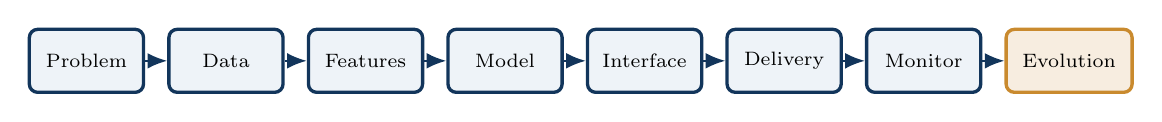
\begin{tikzpicture}[node distance=0.28cm]
  \node[flowbox, minimum width=1.45cm, minimum height=0.8cm] (problem) {\scriptsize Problem};
  \node[flowbox, minimum width=1.45cm, minimum height=0.8cm, right=of problem] (data) {\scriptsize Data};
  \node[flowbox, minimum width=1.45cm, minimum height=0.8cm, right=of data] (features) {\scriptsize Features};
  \node[flowbox, minimum width=1.45cm, minimum height=0.8cm, right=of features] (model) {\scriptsize Model};
  \node[flowbox, minimum width=1.45cm, minimum height=0.8cm, right=of model] (interface) {\scriptsize Interface};
  \node[flowbox, minimum width=1.45cm, minimum height=0.8cm, right=of interface] (delivery) {\scriptsize Delivery};
  \node[flowbox, minimum width=1.45cm, minimum height=0.8cm, right=of delivery] (monitor) {\scriptsize Monitor};
  \node[accentbox, minimum width=1.6cm, minimum height=0.8cm, right=of monitor] (evolution) {\scriptsize Evolution};
  \foreach \a/\b in {problem/data,data/features,features/model,model/interface,interface/delivery,delivery/monitor,monitor/evolution} {
    \draw[arrow] (\a) -- (\b);
  }
  \end{tikzpicture}

  \vspace{0.5em}
  \begin{block}{Today in the course}
  \textbf{Focus:} #1

  \textbf{Bridge:} #2
  \end{block}

  \begin{columns}[T]
  \column{0.48\textwidth}
  \begin{block}{Fraud case}
  {\footnotesize #3}
  \end{block}
  \column{0.48\textwidth}
  \begin{block}{Pasteurization case}
  {\footnotesize #4}
  \end{block}
  \end{columns}

  \vspace{0.3em}
  {\footnotesize \textbf{Course thread:} #5}
  \coursefooter
  \end{frame}
}

\newcommand{\classclosingframe}[4]{
  \begin{frame}{From This Class to the Next}
  \begin{block}{What stays with us}
  #1
  \end{block}

  \begin{columns}[T]
  \column{0.48\textwidth}
  \begin{block}{Project use}
  {\footnotesize #2}
  \end{block}
  \column{0.48\textwidth}
  \begin{block}{Next connection}
  {\footnotesize #3}
  \end{block}
  \end{columns}

  \vspace{0.3em}
  {\footnotesize \textbf{Course thread:} #4}
  \coursefooter
  \end{frame}
}

\tikzset{
  flowbox/.style={
    rounded corners=3pt,
    draw=courseblue,
    fill=courseice,
    very thick,
    minimum width=2.2cm,
    minimum height=0.9cm,
    align=center,
    font=\small
  },
  accentbox/.style={
    rounded corners=3pt,
    draw=coursegold,
    fill=coursegold!15,
    very thick,
    minimum width=2.2cm,
    minimum height=0.9cm,
    align=center,
    font=\small
  },
  arrow/.style={
    -{Latex[length=2.5mm,width=2mm]},
    thick,
    draw=courseblue
  }
}


\title{Class 8: Classes and Object-Oriented Python}
\author{\coursename}
\date{}

\begin{document}

\frame{\titlepage \coursefooter}

\begin{frame}{Agenda}
\begin{itemize}
\item What object-oriented programming actually buys you.
\item Defining a class: \texttt{\_\_init\_\_}, \texttt{self}, attributes, and methods.
\item Class attributes versus instance attributes, and private attributes by convention.
\item Classes you already use every day: \texttt{RandomForestClassifier}, \texttt{StandardScaler}, \texttt{Flask}.
\item Inheritance and why scikit-learn is built on it.
\end{itemize}
\coursefooter
\end{frame}

\begin{frame}{Learning goals}
\learninggoals{
\begin{itemize}
\item Explain what a class, an instance, an attribute, and a method are.
\item Define a small class with a constructor and at least one method.
\item Distinguish class attributes from instance attributes.
\item Recognize that objects you already call --- models, scalers, apps --- are instances of classes.
\item Describe what inheritance provides, using scikit-learn's estimator design as the example.
\end{itemize}
}
\coursefooter
\end{frame}

\coursecontextframe
{Object-oriented programming: bundling data and behavior together.}
{Every function so far has stood alone; a class lets a group of functions share state on purpose.}
{Every time the fraud pipeline writes \texttt{RandomForestClassifier(...)} or \texttt{StandardScaler()}, it is creating an object --- the fraud model itself is an instance of a class.}
{The pasteurization service instantiates \texttt{Flask(\_\_name\_\_)} once and calls methods on that one object for the rest of its life.}
{You have been using classes since Class 5 without naming them; today gives that experience its vocabulary.}

\begin{frame}{What object-oriented programming is}
\begin{itemize}
\item OOP centers on objects that hold both data and the functions that act on that data, in one place.
\item A \textbf{class} is the blueprint; an \textbf{instance} is one concrete object built from that blueprint.
\item A class has \textbf{attributes} (the data an object carries) and \textbf{methods} (the functions it can call on itself).
\item Almost everything in Python is an object --- strings, lists, and functions all have attributes and methods, whether or not you defined their class.
\end{itemize}
\coursefooter
\end{frame}

\begin{frame}[fragile]{Defining a minimal class}
\begin{lstlisting}[style=coursepython]
class SensorReading:
    def __init__(self, name, value):
        self.name = name
        self.value = value

    def describe(self):
        return f"{self.name} = {self.value}"

r = SensorReading("T", 72.0)
print(r.describe())
\end{lstlisting}
\begin{itemize}
\item \texttt{class} starts the definition; \texttt{\_\_init\_\_} is the constructor, run automatically when an instance is created.
\item \texttt{self} refers to the specific instance being built or used; every method takes it as its first parameter.
\end{itemize}
\coursefooter
\end{frame}

\begin{frame}[fragile]{Classes you are already instantiating}
\begin{lstlisting}[style=coursepython]
scaler = StandardScaler()
cls = RandomForestClassifier(n_estimators=200, random_state=42, n_jobs=-1)
app = Flask(__name__)
\end{lstlisting}
\begin{itemize}
\item All three lines, from `streamlit/modeling.py` and `Class6\_model\_api.py`, create an \textbf{instance} of a class you did not write yourself.
\item \texttt{n\_estimators}, \texttt{random\_state}, and \texttt{\_\_name\_\_} are arguments passed straight into that class's \texttt{\_\_init\_\_}.
\end{itemize}
\coursefooter
\end{frame}

\begin{frame}[fragile]{Calling methods on an object}
\begin{lstlisting}[style=coursepython]
cls.fit(X_train_scaled, y_train)
y_pred = cls.predict(X_test_scaled)
app.run(host="0.0.0.0", port=5001, debug=True)
\end{lstlisting}
\begin{itemize}
\item \texttt{.fit(...)}, \texttt{.predict(...)}, and \texttt{.run(...)} are methods: functions that belong to the object and act on its internal state.
\item After \texttt{.fit()}, \texttt{cls} holds a trained model \emph{inside itself} --- that is exactly what attributes are for.
\end{itemize}
\coursefooter
\end{frame}

\begin{frame}{Class attributes versus instance attributes}
\begin{itemize}
\item An \textbf{instance attribute} belongs to one object; it is usually set inside \texttt{\_\_init\_\_} with \texttt{self.name = ...}.
\item A \textbf{class attribute} is defined directly in the class body and is shared by every instance unless overridden.
\item In the example above, every \texttt{SensorReading} has its own \texttt{name} and \texttt{value}; a class attribute would instead be the same for all of them, such as a shared unit label.
\item \texttt{RandomForestClassifier}'s constructor arguments (\texttt{n\_estimators}, \texttt{random\_state}) become instance attributes on \texttt{cls} the moment it is created.
\end{itemize}
\coursefooter
\end{frame}

\begin{frame}{Private attributes, by convention}
\begin{itemize}
\item Python has no strict access control; ``private'' is a naming convention, not enforced by the interpreter.
\item A single leading underscore, \texttt{\_value}, signals ``internal use, please do not touch from outside.''
\item Preferring a method over direct attribute access (a getter, in spirit) keeps the internal representation free to change later.
\item scikit-learn follows this convention itself: attributes set only after \texttt{.fit()}, like \texttt{feature\_names\_in\_}, end with an underscore to mark them as fitted state.
\end{itemize}
\coursefooter
\end{frame}

\begin{frame}{Classes as modules, modules of classes}
\begin{itemize}
\item A class can live in its own \texttt{.py} file, then be imported exactly like the functions in Class 7.
\item Larger projects group related classes into a package: a directory of modules with clear responsibilities.
\item This repository keeps things flatter --- one class per external library call --- but the same organizing principle applies as a project's custom classes grow.
\end{itemize}
\coursefooter
\end{frame}

\begin{frame}[fragile]{Inheritance}
\begin{lstlisting}[style=coursepython]
class Sensor:
    def __init__(self, name):
        self.name = name

    def read(self):
        raise NotImplementedError

class TemperatureSensor(Sensor):
    def read(self):
        return f"{self.name}: reading in degrees C"
\end{lstlisting}
\begin{itemize}
\item Inheritance lets one class reuse and extend another's attributes and methods.
\item \texttt{TemperatureSensor(Sensor)} inherits everything from \texttt{Sensor} and only overrides what needs to differ.
\item \texttt{super().\_\_init\_\_(...)} calls the parent's constructor when the child needs to extend it, not replace it.
\end{itemize}
\coursefooter
\end{frame}

\begin{frame}{Inheritance you rely on without seeing it}
\begin{itemize}
\item Every scikit-learn estimator, \texttt{RandomForestClassifier} included, inherits from common base classes so that \texttt{fit}, \texttt{predict}, and parameter handling behave the same way across the whole library.
\item This shared base is exactly what lets you swap one model class for another and keep calling \texttt{.fit()} and \texttt{.predict()} unchanged --- a theme Class 11 returns to directly.
\item Buitinck et al.\ (2013) document this design choice as central to scikit-learn's API.
\end{itemize}
\coursefooter
\end{frame}

\begin{frame}{How the repo already uses today's building blocks}
\repoactivity{
\begin{itemize}
\item `streamlit/modeling.py` instantiates \texttt{StandardScaler} and \texttt{RandomForestClassifier}, then calls methods on each.
\item `Class6\_model\_api.py` instantiates \texttt{Flask} once at module load and reuses that one object for every route.
\item Find one more class instantiation anywhere in `streamlit/` or `pasteurization/` and name its constructor arguments.
\end{itemize}
}
\coursefooter
\end{frame}

\begin{frame}{Discussion prompt}
\begin{block}{Question}
`RandomForestClassifier` and `StandardScaler` are both instantiated with no custom class ever written for them. When does it actually pay off to write your own class, rather than just calling functions?
\end{block}
\begin{itemize}
\item Pushes past ``because OOP is best practice'' toward a concrete trade-off: shared state and repeated behavior versus added structure.
\end{itemize}
\coursefooter
\end{frame}

\begin{frame}{Papers and materials}
\readinglist{
\href{https://arxiv.org/abs/1309.0238}{Buitinck et al.\ (2013), API design for machine learning software};\
\href{https://scikit-learn.org/stable/}{scikit-learn documentation};\
\href{https://flask.palletsprojects.com/en/stable/}{Flask documentation}.
}
\coursefooter
\end{frame}

\classclosingframe
{\begin{itemize}
\item Classes bundle data and behavior; instances are the concrete objects built from that blueprint.
\item \texttt{self}, \texttt{\_\_init\_\_}, and methods are the syntax; attributes carrying state are the payoff.
\item You were already using classes --- scikit-learn's and Flask's --- well before today's vocabulary caught up.
\end{itemize}}
{Before writing more script-level code for your project, ask whether related state and behavior should be grouped into a class instead.}
{Class 9 turns back to data itself: loading, indexing, and light cleaning with pandas on a real dataset.}
{Objects hold state; next class is about the state --- the data --- those objects will eventually operate on.}

\end{document}
